\chapter{Tecnologias \textit{Web}}

\section{\textit{Framework}}
Segundo \citeonline{artigo_oo_reuso_software}, a programação orientada a objetos é muita vezes utilizada para promover o reuso de software. Para \citeonline{artigo_reuso_classes}, algumas linguagens, como \textit{Smalltalk}, são utilizadas tanto para reduzir o tempo de desenvolvimento quanto o custo de manutenção, simplificando a criação de novos sistemas e de novas versões para sistemas já existentes. Afirma, também, que ``componentes de um programa devem ser projetados para reusabilidade''.

Os mesmos autores confirmam que um ``design abstrato orientado a objetos'', também chamado de \textit{framework}, define uma interface para os principais componentes dentro de uma
arquitetura pré-definida. ``\textit{Frameworks} provêem uma maneira de reutilizar código que é resistente a mais tentativas de reusos convencionais''.

\citeonline{artigo_reuso_classes}, comparam ``programas esqueletos'' com \textit{frameworks}, os quais consistem em uma abordagem tradicional de reutilização de código e na garantia de consistência entre todos os componentes de um sistema sobre a mudança de algum requisito. O autor também realiza uma comparação entre os \textit{frameworks} do tipo ``caixa-branca'' e ``caixa-preta'', o primeiro é responsável por especificar o comportamento de uma aplicação adicionando-se métodos para subclasses de uma ou mais de suas classes, ou seja, a implementação deste tipo de \textit{framework} deve ser conhecida para sua utilização, o segundo consiste no uso de um protocolo responsável por definir uma interface entre os componentes,. Deste modo, o usuário precisaria entender apenas como funciona a interface externa dos componentes para utilizá-los.

\section{\textit{Django}}
O \textit{Django} \cite{django_project} é um \textit{framework} para desenvolvimento \textit{web} implementado na linguagem Python\footnote{\url{https://www.python.org/}}. Sua arquitetura inspira-se no modelo tradicional MVC(\textit{Model} \textit{View} \textit{Controller}), porém, com algumas especificidades. A comunidade \textit{Django} adota o acrônimo MTV (\textit{Model} \textit{Template} \textit{View}), onde os papéis de \textit{model}, \textit{view} e \textit{controller} são redefinidos como:
\begin{itemize}
    \item \textit{Model}: corresponde à \textit{model} do MVC tradicional e representa as classes que popularão as tabelas do banco de dados. O \textit{Django} possui um ORM (\textit{Object-Relational Mapping}, Mapeamento de Objeto Relacional) para realizar a manipulação dessas tabelas, não sendo necessário a escrita de consultas em SQL para a persistência das informações.
    \item \textit{Template}: corresponde aproximadamente à \textit{view} do MVC tradicional e descreve como as informações serão apresentadas para o usuário.
    \item \textit{View}: representada por uma função \textit{callback} referente à uma classe de URLs, descrevendo quais informações serão apresentadas e como elas serão enviadas para o \textit{template}. Alguns autores defendem que a view corresponde ao \textit{controller} do MVC tradicional, mas os próprios desenvolvedores do \textit{Django} a \textit{view} deve ser minimalista e boa parte do papel do \textit{controller} deve ser implementado nas próprias classes dos modelos.
\end{itemize}

Na nomenclatura do \textit{Django}, um conjunto de funcionalidades pode ser agrupado em aplicação. Cada aplicação possui suas próprias \textit{models}, \textit{views} e \textit{templates}.

A Figura \ref{django-arq} mostra a arquitetura do \textit{Django}, apresentando as camadas do MTV durante a comunicação com o navegador até o acesso ao banco de dados. O \textit{URL dispatcher} identifica endereços requisitados pelo usuário e realiza o redirecionamento da requisição para a aplicação correta. A coordenação de requisições entre o \textit{URL dispatcher} e a \textit{view} e da \textit{view} até o \textit{template} é feita pelos chamados \textit{Middlewares}. Os \textit{Middlewares} realizam a persistência de informações entre as diferentes camadas.

\begin{figure}[h]
    \centering
    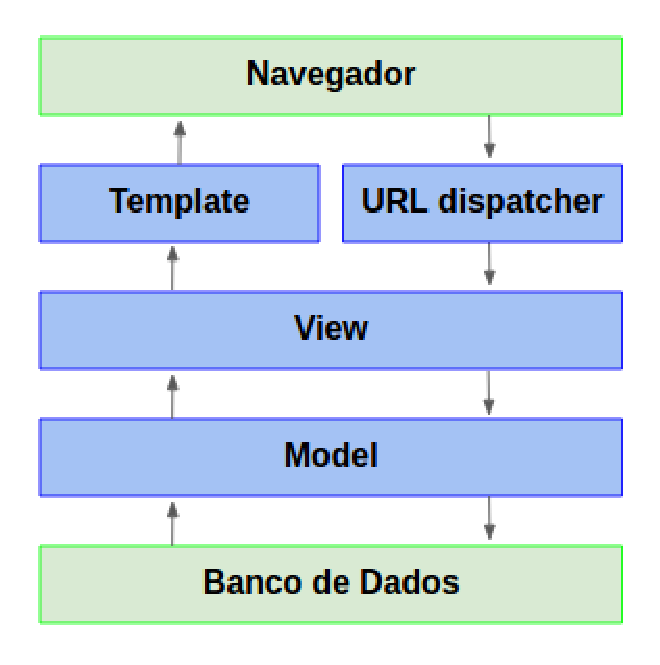
\includegraphics[keepaspectratio=true,scale=0.5]{figuras/django-arquitetura.eps}
    \caption{Arquitetura MTV \textit{Django}}
    \label{django-arq}
\end{figure}

\section{Ferramentas \textit{Web} Utilizadas}
    \subsection{\textit{Coverage}}
    Coverage\footnote{\url{https://pypi.python.org/pypi/coverage/}} é uma ferramenta python responsável por medir a cobertura de código para o conjunto de testes unitários utilizado. A ferramentas rastreia quais linhas de código foram executadas pela suíte de testes.

    \subsection{\textit{GitLab CI}}
    \textit{GitLab CI}\footnote{\url{https://about.gitlab.com/gitlab-ci/}} ferramenta integrada ao {GitLab} para realizar serviços de integração contínua a cada \textit{commit}. A integração contínua está configurada para instalar as dependências do projeto, executar a suíte de testes e verificação de estilo com flake8\footnote{url{https://pypi.python.org/pypi/flake8}}.

    \subsection{\textit{Django-Cron}}
    \textit{Django-Cron}\footnote{\url{http://django-cron.readthedocs.io/en/latest/index.html}} é uma ferramenta para execução de \textit{scripts} em \textit{python} de forma temporizada.

    \subsection{\textit{Sphinx}}
    \textit{Sphinx}\footnote{\url{http://www.sphinx-doc.org/}} é uma ferramenta para criação inteligente e estilizada de documentação de códigos em \textit{python}, C/C++
    e outras linguagens. Utiliza \textit{reStructuredText}\footnote{\url{http://docutils.sourceforge.net/rst.html}} como sua linguagem de marcação e converte toda a documentação para formato html, pdf, epub ou man.

\section{Protocolos Utilizados}
    \subsection{\textit{Modbus RTU}}
    \textit{Modbus} é um protocolo serial utilizado para transmitir informações entre dispositivos eletrônicos. Suas mensagens utilizam a arquitetura de mestre-escravo, como mostrado na figura \ref{mestre_escravo} \cite{modbus}. Nesta arquitetura, o papél de mestre é designado ao dispositivo que envia as requisições e escravo ao que responde passivamente às mesmas.

    \begin{figure}[!htpb]
        \centering
        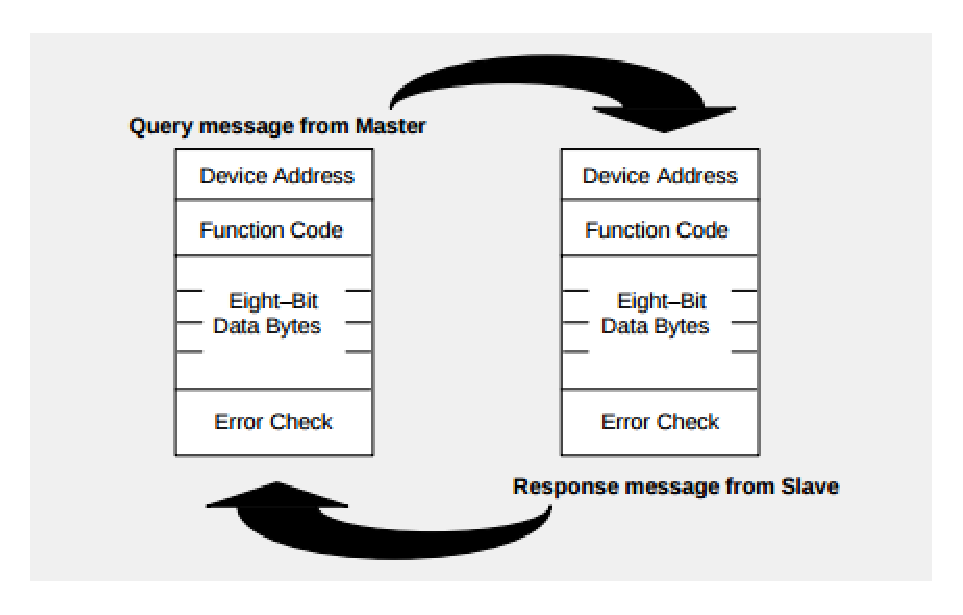
\includegraphics[keepaspectratio=true,scale=0.8]{figuras/mestre_escravo.eps}
        \caption{Comunicação Mestre-Escravo \textit{Modbus}. Fonte: \cite{modbus}}
        \label{mestre_escravo}
    \end{figure}

    Quando controladores são configurados para se comunicarem em uma rede Modbus usando o modo RTU (\textit{Remote Terminal Unit}, Unidade de Terminal Remoto) cada \textit{byte} contém duplas hexadecimais de 4 \textit{bits}. A maior vantagem de utilizar este modo é que sua grande densidade de caracteres permite uma maior taxa de transferência comparado ao modo ASCII em uma mesma taxa de transmissão \cite{modbus}.

    Uma mensagem em Modbus RTU possui 16 \textit{bytes} e é definida da seguinte maneira:
    \begin{itemize}
        \item Identificador do Aparelho: 2 \textit{bytes}.
        \item Código de Função: 2 \textit{bytes}, define qual tipo de operação o equipamento irá realizar.
        \item Campo de Dados: 8 \textit{bytes}, sendo 4 \textit{bytes} para indicar o endereço do primeiro registrador requisitado e 4 \textit{bytes} para indicar a quantidade de registradores que serão lidos.
        \item CRC (\textit{Cyclic Redundancy Check}, Verificação de Redundância Cíclica): 4 \textit{bytes} para verificação de erros.
    \end{itemize}

    A resposta do escravo possui a seguinte estrutura:

    \begin{itemize}
        \item Identificador do Aparelho: 2 \textit{bytes}.
        \item Código de Função: 2 \textit{bytes}, define qual tipo de operação o equipamento irá realizar.
        \item Tamanho do{payload}: 2 \textit{bytes}, define o tamanho do campo de dados em \textit{bytes}.
        \item Campo de dados: possui tamanho variável, de acordo com o valor do campo anterior.
        \item CRC (\textit{Cyclic Redundancy Check}, Verificação de Redundância Cíclica): 4 \textit{bytes} para verificação de erros.
    \end{itemize}

    \subsection{UDP}
    O protocolo UDP (\textit{User Datagram Protocol}, Protocolo de Datagrama do Usuário) é um protocolo da camada de transporte e não orientado a conexões. Seu cabeçalho, figura \ref{udp_header}, possui 8 \textit{bytes}, seguido de uma carga útil. As portas apresentadas no cabeçalho representam as máquinas de origem e destino \cite{tanenbaum_2002}.

    \begin{figure}[!htpb]
        \centering
        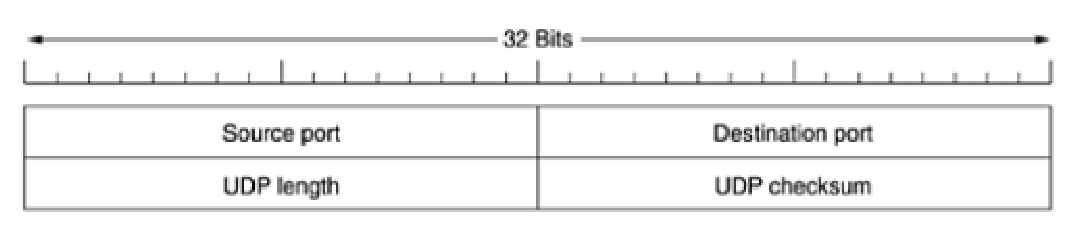
\includegraphics[keepaspectratio=true,scale=0.8]{figuras/udp_header.eps}
        \caption{Cabeçalho do UDP. Fonte: \cite{tanenbaum_2002}}
        \label{udp_header}
    \end{figure}

    O protocolo \textit{Modbus RTU} é encapsulado no campo de dados do protocolo UDP. Neste encapsulamento, o endereço ModBus de todos os equipamentos é igual a 1, sendo que a diferenciação entre equipamentos se dá pelo número de IP.